\section{Approach}
	In this section we will present our aproach to tackle the speaker recognition problem.
\subsection{Erollment}
	\label{sec:approach_enrollment}
	An continuous speech of a user is collected during enrollment of that user. Depending on
	the number of users we plan to enroll and the accuracy of recognition system, duration
	of the utterance we need to collect may vary from 15 seconds to 30 seconds.

	Further processing of the utterance follows following steps:
	\begin{enumerate}
		\item \textbf{Voice Activity Detection (VAD)} \\
			Due to the channel difference and background noise may occur, which
			may degrade the performance of the system, non-speech part of the
			speech are removed from the utterance. This may lead to
			information loss (such as person's voice pause style), which in
			turns introduced the trade-off between loss of information and
			noise been modeled.

			As the corpus provided by teacher is nearly noise-free, we use a
			simple energy-based approach to remove the silence part.

		\item \textbf{Extract MFCC feature representation} \\
			The utterance is then transformed to MFCC features with $20ms$
			frame-duration and $10ms$ frame-shift. Further more, we tuned the
			parameters of MFCC to yield better result. 40 filter banks and 19
			cepstral coefficent are parameters found to perform best.

			We have extensively examined MFCC feature. We found that, the
			distribution of a person's MFCC feature is truly a good representation
			of its vocal characteristics. Here are some plots of the first three
			dimensions of a spearker's MFCC feature.
			\begin{figure}[!ht]
				\begin{minipage}{0.48\linewidth}
					\centering
					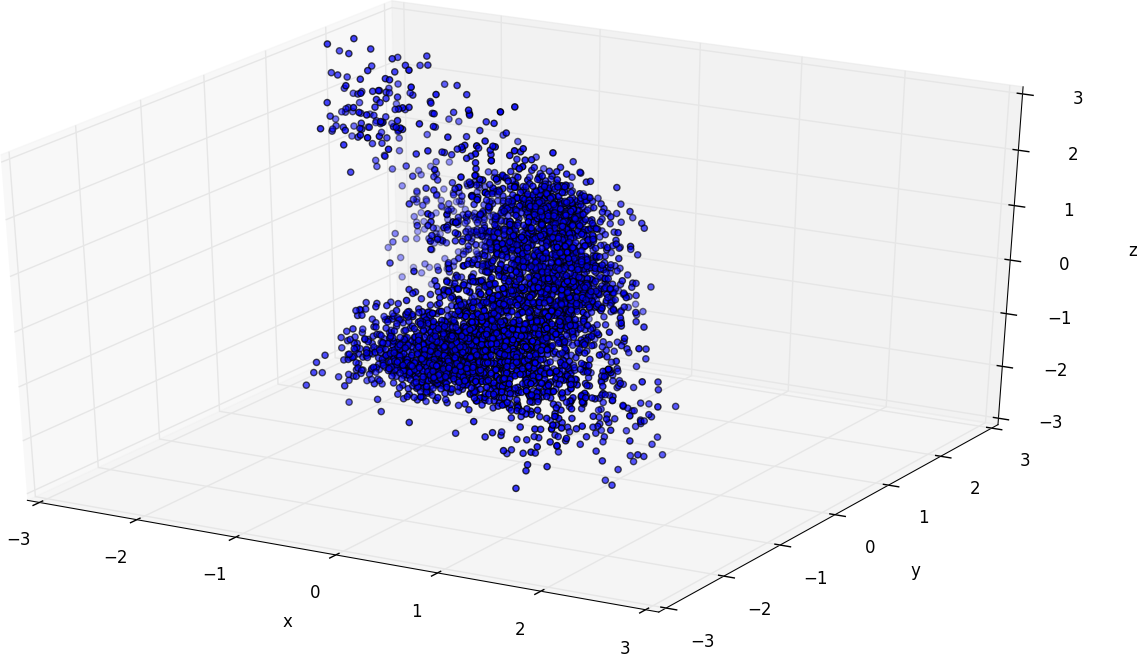
\includegraphics[width=\linewidth]{res/m_002_03.trimed.png}
					\caption{The first three dimension of a man's MFCC feature}
				\end{minipage}
				\hfill
				\begin{minipage}{0.48\linewidth}
					\centering
					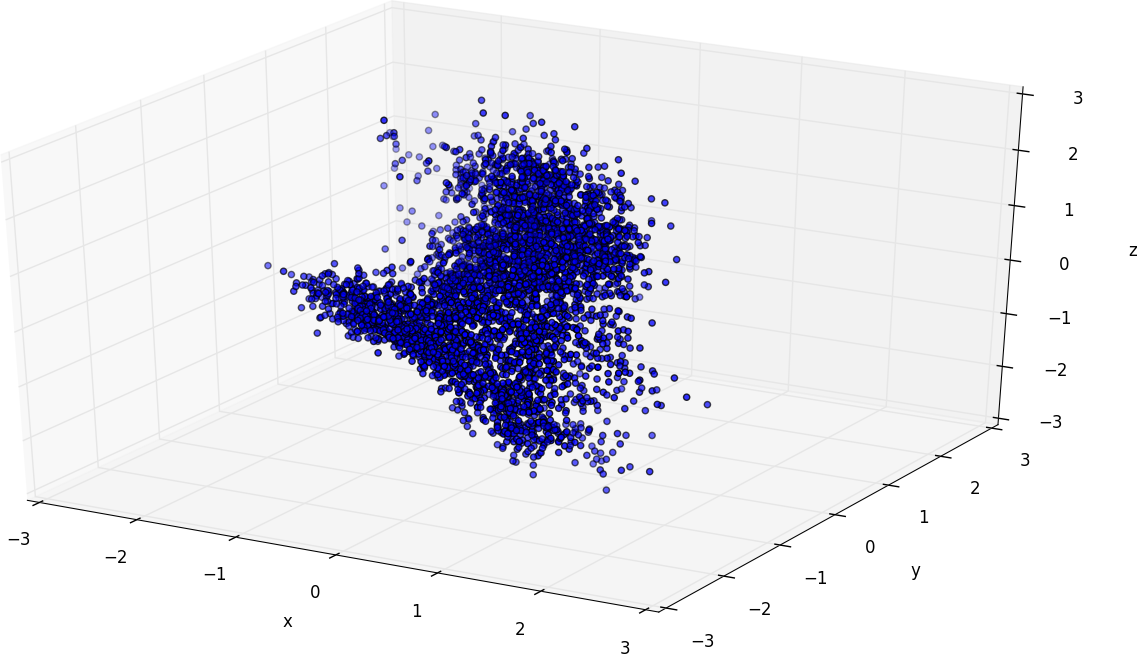
\includegraphics[width=\linewidth]{res/m_004_03.trimed.png}
					\caption{The first three dimension of another man's MFCC feature}
				\end{minipage}
				\vfill
				\begin{minipage}{0.48\linewidth}
					\centering
					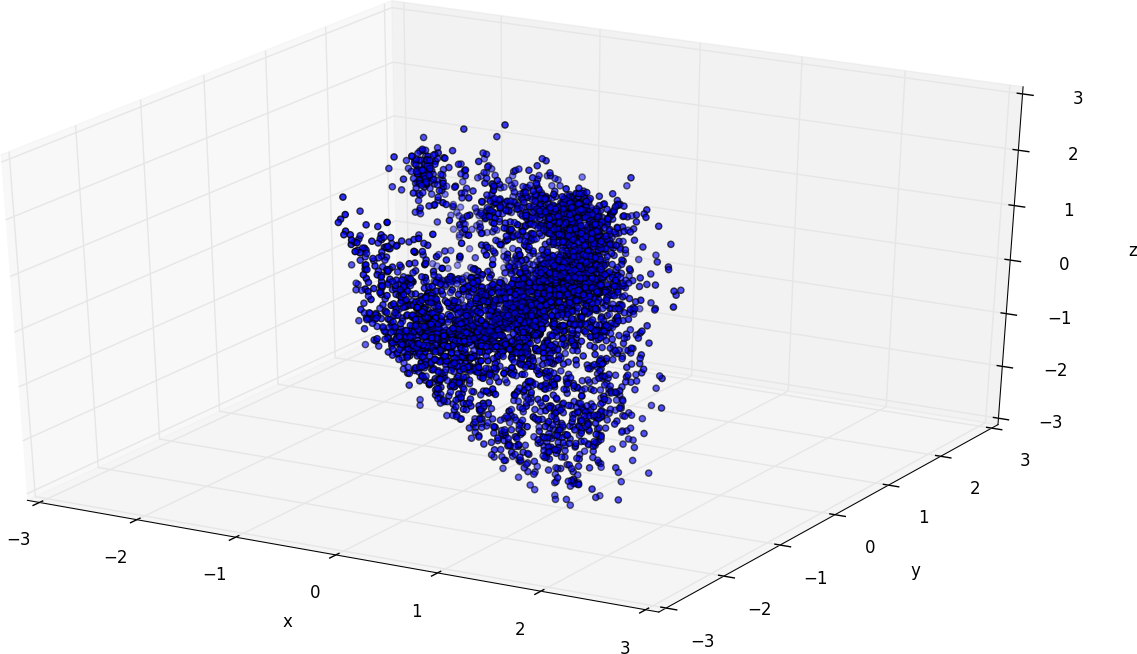
\includegraphics[width=\linewidth]{res/f_001_03.trimed.png}
					\caption{The first three dimension of a woman's MFCC feature}
				\end{minipage}
				\hfill
				\begin{minipage}{0.48\linewidth}
					\centering
					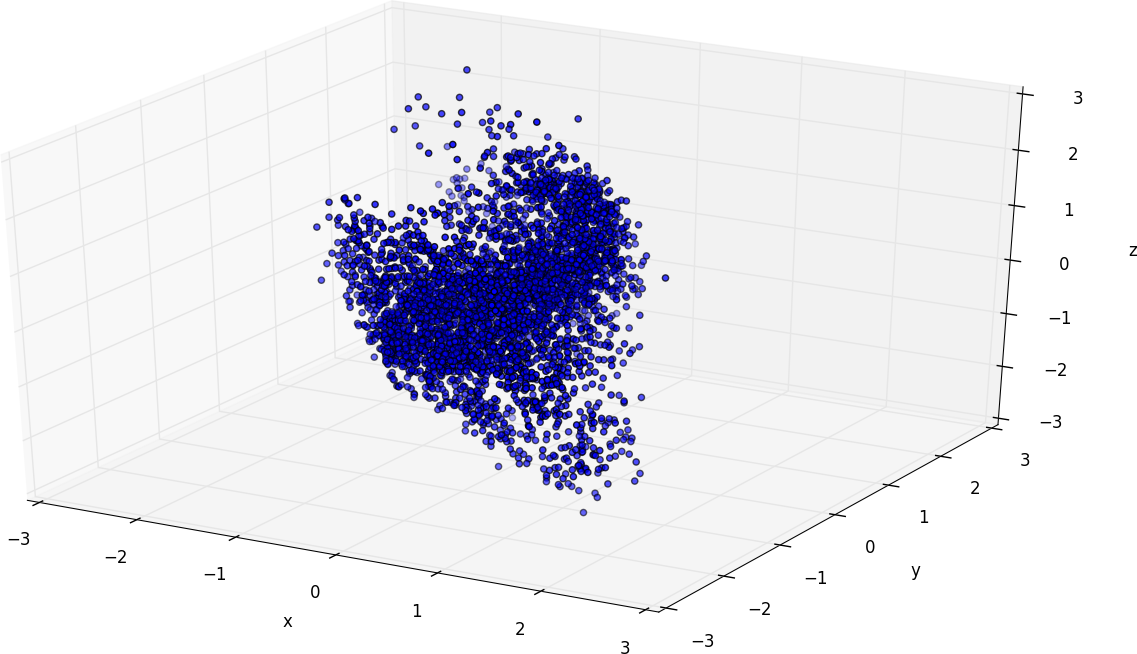
\includegraphics[width=\linewidth]{res/f_003_03.trimed.png}
					\caption{The first three dimension of another woman's MFCC feature}
				\end{minipage}
			\end{figure}

			It is clearly showed in the figure that, women's MFCC feature distribution
			tends to have nice ecliptical shapes in first three-dimension,
			as women's voice pitch is higher than man. And the two men's MFCC figure
			shows great difference on density over space. It shows high correspondency
			of the theoretical analysis.

		\item \textbf{Gaussian Mixture Model} \\
			As the MFCC feature of a utterance of a user is a high-dimensional point
			set, which comprised a distribution, we model a user by modeling its
			MFCC feature distribution. The generative model we have primally adopted is
			Gaussian Mixture Model(GMM).

			In order to conduct a proof-of-concept experiments, we consequently conducted
			experiments using GMM from \textit{scikit-learn}\cite{scikit-learn}
			and \textit{PyPR}\cite{pypr}, but it turns out that these implementations
			are neither of efficiency, nor of decent accuracy. Therefore, we implemented
			our own GMM model with following improvements:
			\begin{itemize}
				\item As GMM is very sensitive to initialization, we use
					K-Means to initialize the configuration prior to GMM training.

				\item Further more, we use an improved algorithm of
					K-means++\cite{arthur2007k} named K-meansII\cite{bahmani2012scalable},
					which outperforms both naive K-means and K-means++ in both
					efficiency and accuracy. For detailed algorithm description,
					please consult the orignal paper.

				\item All above algorithms (K-means, K-means++, K-meansII and
					GMM) are implemented utilizing multi-core CPUs in
					thread level. Experiments shows that our implementation
					scales nearly linearly with number of cores.

				\item In order to futher speed up the training process,
					we examined the time consuming part of GMM algorithm,
					which lies in extensive use of exponential function.
					Therefore, we rewrite exponential function using 5-order polynomial
					approximation using \textbf{SSE} instructions, which only
					introduced an numerical error less than $10^{-7}$.
					The running time of the training process cut by half when using
					our optimization.
			\end{itemize}

			Using these optimizations, our GMM training is at least \textbf{300
			times} faster than that of PyPR \cite{pypr}
			\footnote{
				This is an rough estimation which highly biased to PyPR. The factor 300
				is estimated by the average running time of one iteration when training GMM
				using PyPR (30 miniutes) divides the longest iteration time of our
			GMM (which is 6 seconds)}
			when training Universal Background Model(UBM) using 14 cores.

			Further more, our implementation of GMM outperforms the GMM library
			aforementioned by $1\%$ in terms of recognition accuracy.

		\item \textbf{Continuous restricted Boltzmann Machine(CRBM)}
			Restricted Boltzmann Machine(RBM) is generative stochastic neural
			network that can learn a probability distribution over its set of
			inputs\cite{rbm_wiki}. But original version of RBM can only deal
			with binary inputs. \cite{chen2003continuous} proposed and extension called
			Continuous restricted Boltzmann Machine, which can deal with real-valued
			inputs. RBM is a two-layer neural network, in which one layer called
			visible layer (the input), and another called hidden layer. The neurons
			in hidden layer controls the model complexity and the performance of
			the network. Both RBM and CRBM can be trained using Contrastive
			Divergence learning.

			RBM has the ability of given an input(visible layer), reconstruct a visible
			layer that is similar to the input. This demonstrates the modeling ability
			of RBM. \figref{crbm} illustrate original MFCC data and the sampled output of
			reconstructed data from CRBM.
			\begin{figure}[!ht]
				\label{fig:crbm}
				\begin{minipage}{0.48\linewidth}
					\centering
					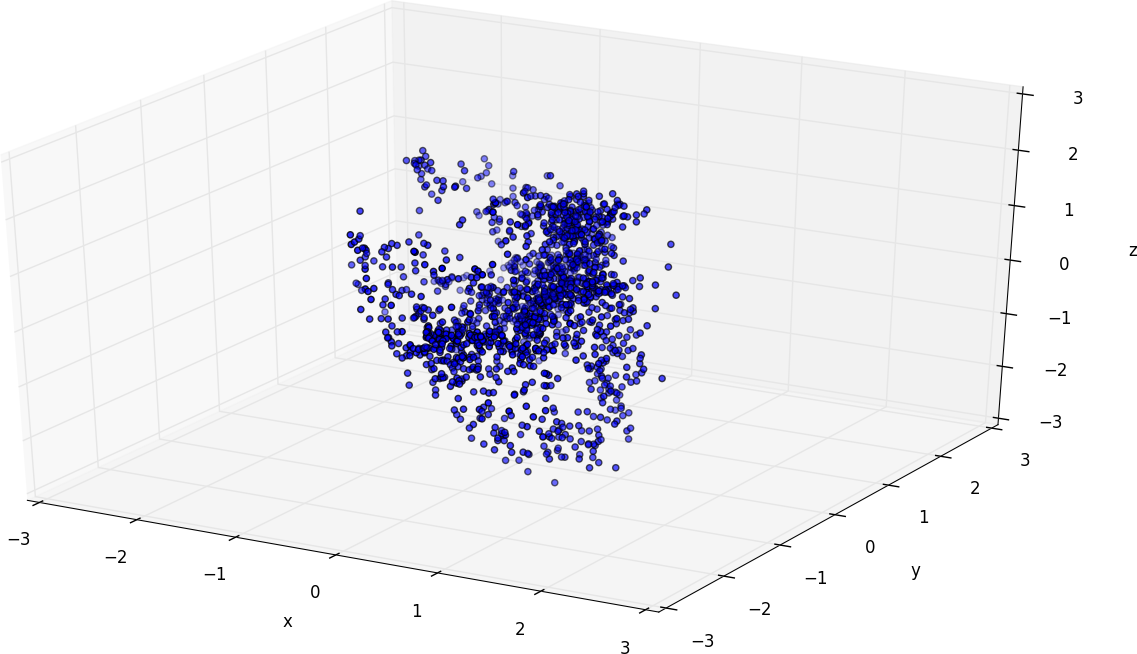
\includegraphics[width=\linewidth]{res/all.trimed.png}
					\caption{The first three dimension of a man's MFCC feature}
				\end{minipage}
				\hfill
				\begin{minipage}{0.48\linewidth}
					\centering
					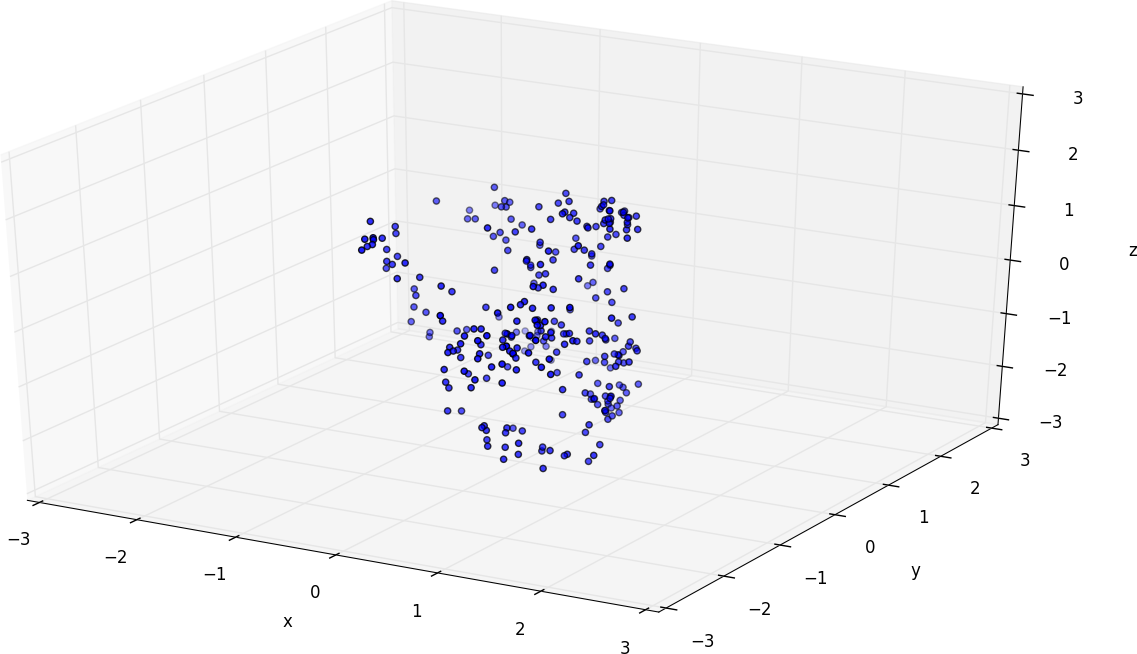
\includegraphics[width=\linewidth]{res/50.trimed.png}
					\caption{The first three dimension of the same man's MFCC feature
					recontructed by a CRBM with 50-neuron hidden layer. We can
					see that, the density of these two distributions are alike}
				\end{minipage}
			\end{figure}

		\item \textbf{JFA}:

          \textbf{Factor Analysis} is a typical method which behave
          very well in classification problems, due to its ability to
          account for different types of variability in training data.
          Within all the factor analysis methods,
          Joint Factor Analysis (JFA)\cite{jfa2,jfa-se} was proved to outperform other method
          in the task of Speaker Recognition.

          JFA models the user by ``supervector'' , i.e. a $C\times F $ dimension vector, where $C$ is
          the number of components in the Universal Background Model, trained by GMM on all the training data,
          and $ F$ is the dimension of the acoustic feature vector. The supervector of an utterance is obtained by concatenate
          all the $C $ means vectors in the trained GMM model. The basic assumption of JFA on describing a supervector is:

          \[ \vec{M} = \vec{ m } + vy + dz + ux, \]

          where $m$ is a supervector usually selected to be the one trained from UBM, $v$ is a $ CF \times R_s$ dimension matrix,
          $ u$ is a $ CF \times R_c$ dimension matrix, and $d$ is a diagonal matrix.
          This four variables are considered independent of all kinds of variabilities and remain constant after training, and
          $x, y, z $ are matrixes computed for each utterance sample.
          In this formulation, $ m + vy + dz$ is commonly believed to account for the ``Inter-Speaker Variability'', and $ux $ accounts
          for the ``Inter-Channel Variability''.
          The parameter $ R_s $ and $ R_c$, also referred to as ``Speaker Rank'' and ``Channel Rank'', are two emprical constant selected as first.
          The training of JFA is to calculate the best $ u, v, d$ to fit all the training data.

          However, the original algorithm \cite{jfa-se} for training JFA model is of
          too much complication and hard to implement.
          Therefore, we use the simpler algorithm presented in \cite{jfa-study}

          to train the JFA model.
	\end{enumerate}

\subsection{Recognition}
	Recognition procedure follows steps below:
	\begin{enumerate}
		\item Record a short utterance of the speaker (typically 5 seconds)
		\item Preprocess the utterance using first two steps described in
			\secref{approach_enrollment}, e.g, VAD and MFCC feature extraction.
		\item Compute the `score' of the MFCC featuresextraced for each model of persons
			enrolled, and adopt person corresponding the model which gives highest score to be the
			recognition result.

			A typical form of score is log-likelihood (or enery in RBM case).

	\end{enumerate}

